\documentclass[12pt,a4paper]{article}
\usepackage{ctex}
\usepackage{amsmath,amscd,amsbsy,amssymb,latexsym,url,bm,amsthm}
\usepackage{epsfig,graphicx,subfigure}
\usepackage{enumitem,balance}
\usepackage{wrapfig}
\usepackage{listings}
\usepackage{mathrsfs,euscript}
\usepackage[usenames]{xcolor}
\usepackage{hyperref}
\usepackage[vlined,ruled,linesnumbered]{algorithm2e}
\usepackage{array}
\hypersetup{colorlinks=true,linkcolor=black}

\newtheorem{theorem}{Theorem}
\newtheorem{lemma}[theorem]{Lemma}
\newtheorem{proposition}[theorem]{Proposition}
\newtheorem{corollary}[theorem]{Corollary}
\newtheorem{exercise}{Exercise}
\newtheorem*{solution}{Solution}
\newtheorem{definition}{Definition}
\theoremstyle{definition}

\renewcommand{\thefootnote}{\fnsymbol{footnote}}

\newcommand{\postscript}[2]
 {\setlength{\epsfxsize}{#2\hsize}
  \centerline{\epsfbox{#1}}}

\renewcommand{\baselinestretch}{1.0}

\setlength{\oddsidemargin}{-0.365in}
\setlength{\evensidemargin}{-0.365in}
\setlength{\topmargin}{-0.3in}
\setlength{\headheight}{0in}
\setlength{\headsep}{0in}
\setlength{\textheight}{10.1in}
\setlength{\textwidth}{7in}
\makeatletter \renewenvironment{proof}[1][Proof] {\par\pushQED{\qed}\normalfont\topsep6\p@\@plus6\p@\relax\trivlist\item[\hskip\labelsep\bfseries#1\@addpunct{.}]\ignorespaces}{\popQED\endtrivlist\@endpefalse} \makeatother
\makeatletter
\renewenvironment{solution}[1][Solution] {\par\pushQED{\qed}\normalfont\topsep6\p@\@plus6\p@\relax\trivlist\item[\hskip\labelsep\bfseries#1\@addpunct{.}]\ignorespaces}{\popQED\endtrivlist\@endpefalse} \makeatother

\begin{document}
\noindent

%========================================================================
\noindent\framebox[\linewidth]{\shortstack[c]{
\Large{\textbf{Lab10-Turing Machine}}\vspace{1mm}\\
Algorithm and Complexity (CS214), Xiaofeng Gao, Spring 2020.}}
\begin{center}
\footnotesize{\color{red}$*$ If there is any problem, please contact TA Yiming Liu. }

\footnotesize{\color{blue}$*$ Name:Hongjie Fang  \quad Student ID:518030910150 \quad Email: galaxies@sjtu.edu.cn}
\end{center}

\begin{enumerate}

\item
Design a one-tape TM $M$ that computes the function $f(x, y) = x \mod y$, where $x$ and $y$ are positive integers ($x > y$). The alphabet is $\{1, 0, \Box, \triangleright, \triangleleft\}$, and the inputs are $x$ 1's, $\Box$ and $y$ 1's. Below is the initial configuration for input $x=7$ and $y=3$. The result $z=f(x, y)$ should also be represented in the form of $z$ 1's on the tape with the pattern of $\triangleright 111 \cdots 111 \triangleleft$.
\begin{center}
	\begin{tabular}{ll|c|c|c|c|c|c|c|c|c|c|c|c|c|c}
		& \multicolumn{14}{c}{Initial Configuration}\\[5pt]
		\cline{2-16}
		& & $\triangleright$ &  1  & 1 & 1 & 1 & 1 & 1 & 1 & $\Box$ & 1 & 1 & 1 & $ \triangleleft$ & \\
		\cline{2-16}
		\multicolumn{2}{c}{} & \multicolumn{1}{c}{$\uparrow$} & \multicolumn{11}{c}{}\\[-4px]
		\multicolumn{2}{c}{} & \multicolumn{1}{c}{$q_S$} & \multicolumn{11}{c}{}	
	\end{tabular}
\end{center}

\begin{enumerate}
	\item
	Please describe your design and then write the specifications of $M$ in the form like $\langle q_S, \triangleright \rangle \rightarrow \langle q_1, \triangleright,  R\rangle$. Explain the transition functions in detail.
	
	\item
	Please draw the state transition diagram.
	
	\item
	Show briefly and clearly the whole process from initial to final configurations for input $x = 7$ and $y = 3$. You may start like this:
	$$(q_s,\underline{\triangleright}  1  1  1  1  1  1  1  \Box 1  1  1   \triangleleft)
	\vdash (q_1,\triangleright  \underline{1}  1  1  1  1  1  1  \Box 1  1  1   \triangleleft)
	\vdash^* (q_1,\triangleright  1  1  1  1  1  1  1  \underline{\Box} 1  1  1   \triangleleft)
	\vdash (q_2,\triangleright  1  1  1  1  1  1  1  \Box \underline{1}  1  1   \triangleleft)$$
	
	\par{\color{blue}(Note that for simplicity, we write $(q_1,\triangleright  \underline{1}  1  1  1  1  1  1  \Box 1  1  1   \triangleleft)\vdash^* (q_1,\triangleright  1  1  1  1  1  1  1  \underline{\Box} 1  1  1   \triangleleft)$ if the corresponding transaction repeats on multiple inputs with the same state.)}
	
\end{enumerate}
\begin{solution}
Here are my answers to the sub-questions.
\begin{enumerate}
\item Here are the specific transitions of $M$:
\begin{displaymath}
\begin{aligned}
& \langle q_S, \triangleright \rangle \rightarrow \langle q_1, \triangleright, R\rangle & \\
& \langle q_1, 1 \rangle \rightarrow \langle q_1, 1, R\rangle & \qquad
& \langle q_1, \Box \rangle \rightarrow \langle q_1, \Box, R\rangle & \qquad
& \langle q_1, \triangleleft \rangle \rightarrow \langle q_2, \triangleleft, L\rangle & \\
& \langle q_2, 1 \rangle \rightarrow \langle q_3, \triangleleft, L\rangle &
& \langle q_2, \Box \rangle \rightarrow \langle q_5, 1, L\rangle & \\
& \langle q_3, 1 \rangle \rightarrow \langle q_3, 1, L\rangle & \qquad
& \langle q_3, \Box \rangle \rightarrow \langle q_4, \Box, L\rangle & \\
& \langle q_4, 1 \rangle \rightarrow \langle q_1, \Box, R\rangle & \qquad
& \langle q_4, \Box \rangle \rightarrow \langle q_4, \Box, L\rangle & \qquad
& \langle q_4, \triangleright \rangle \rightarrow \langle q_7, \triangleright, R\rangle & \\
& \langle q_5, 1 \rangle \rightarrow \langle q_6, 1, R\rangle & \qquad
& \langle q_5, \Box \rangle \rightarrow \langle q_5, 1, L\rangle & \qquad
& \langle q_5, \triangleright \rangle \rightarrow \langle q_6, \triangleright, R\rangle & \\
& \langle q_6, 1 \rangle \rightarrow \langle q_1, \Box, R\rangle & \\
& \langle q_7, 1 \rangle \rightarrow \langle q_8, 1, L\rangle & \qquad
& \langle q_7, \Box \rangle \rightarrow \langle q_7, 1, R\rangle & \qquad
& \langle q_7, \triangleleft \rangle \rightarrow \langle q_8, \triangleleft, L\rangle & \\
& \langle q_8, 1 \rangle \rightarrow \langle q_h, \triangleleft, S\rangle & \\
\end{aligned}
\end{displaymath}

\textbf{(Method Explanation)} The main method of my design is that we repeat trying to \underline{eliminate $y$ ``1''s in $x$'s representation, until there is not enough ``1''s in $x$'s representation}, and the rest of ``1''s in $x$'s representation are the result of $x\mod y$. What's more, we \underline{do not use ``0'' in the design of the Turing Machine}; therefore it also works on a simple alphabet $\Gamma'=\{1, \Box, \triangleright, \triangleleft\}$.

\textbf{(Transitions Explanations)} Here are some detailed explanations.
\begin{itemize}
\item[\textbf{Step 1.} ] Find out the last ``1'' in the representation of $y$ using the following transitions:
\begin{displaymath}
\begin{aligned}
& \langle q_S, \triangleright \rangle \rightarrow \langle q_1, \triangleright, R\rangle & \\
& \langle q_1, 1 \rangle \rightarrow \langle q_1, 1, R\rangle & \qquad
& \langle q_1, \Box \rangle \rightarrow \langle q_1, \Box, R\rangle & \qquad
& \langle q_1, \triangleleft \rangle \rightarrow \langle q_2, \triangleleft, L\rangle & \\
\end{aligned}
\end{displaymath}

\item[\textbf{Step 2a.} ] If found, change this ``1'' to ``$\triangleleft$'' using the following transition, and go to Step 3.
\begin{displaymath}
\langle q_2, 1 \rangle \rightarrow \langle q_3, \triangleleft, L\rangle
\end{displaymath}

\item[\textbf{Step 2b.} ] If not found, change all the ``$\Box$'' except the first to ``1'' using the following transitions, and go back to Step 1.
\begin{displaymath}
\begin{aligned}
& \langle q_2, \Box \rangle \rightarrow \langle q_5, 1, L\rangle & \\
& \langle q_5, 1 \rangle \rightarrow \langle q_6, 1, R\rangle & \qquad
& \langle q_5, \Box \rangle \rightarrow \langle q_5, 1, L\rangle & \qquad
& \langle q_5, \triangleright \rangle \rightarrow \langle q_6, \triangleright, R\rangle & \\
& \langle q_6, 1 \rangle \rightarrow \langle q_1, \Box, R\rangle & \\
\end{aligned}
\end{displaymath}

\item[\textbf{Step 3.} ] Find out the last ``1'' in the representation of $x$ using the following transitions.
\begin{displaymath}
\begin{aligned}
& \langle q_3, 1 \rangle \rightarrow \langle q_3, 1, L\rangle & \quad
& \langle q_3, \Box \rangle \rightarrow \langle q_4, \Box, L\rangle & \\
& \langle q_4, \Box \rangle \rightarrow \langle q_4, \Box, L\rangle &
\end{aligned}
\end{displaymath}

\item[\textbf{Step 4a.} ] If found, change this ``1'' to ``$\Box$'' using the following transition, and go to Step 1.
\begin{displaymath}
\langle q_4, 1 \rangle \rightarrow \langle q_1, \Box, R\rangle
\end{displaymath}

\item[\textbf{Step 4b.} ] If not found, change all the ``$\Box$'' except the last to ``1'' and change the last to ``$\triangleleft$'' using the following transitions, and the process is finished.
\begin{displaymath}
\begin{aligned}
& \langle q_4, \triangleright \rangle \rightarrow \langle q_7, \triangleright, R\rangle & \\
& \langle q_7, 1 \rangle \rightarrow \langle q_8, 1, L\rangle & \qquad
& \langle q_7, \Box \rangle \rightarrow \langle q_7, 1, R\rangle & \qquad
& \langle q_7, \triangleleft \rangle \rightarrow \langle q_8, \triangleleft, L\rangle & \\
& \langle q_8, 1 \rangle \rightarrow \langle q_h, \triangleleft, S\rangle & \\
\end{aligned}
\end{displaymath}
\end{itemize}
\item The state transition diagram of my Turing Machine is as follows (Fig. \ref{fig1}).
\begin{figure}[htbp]
  \centering
  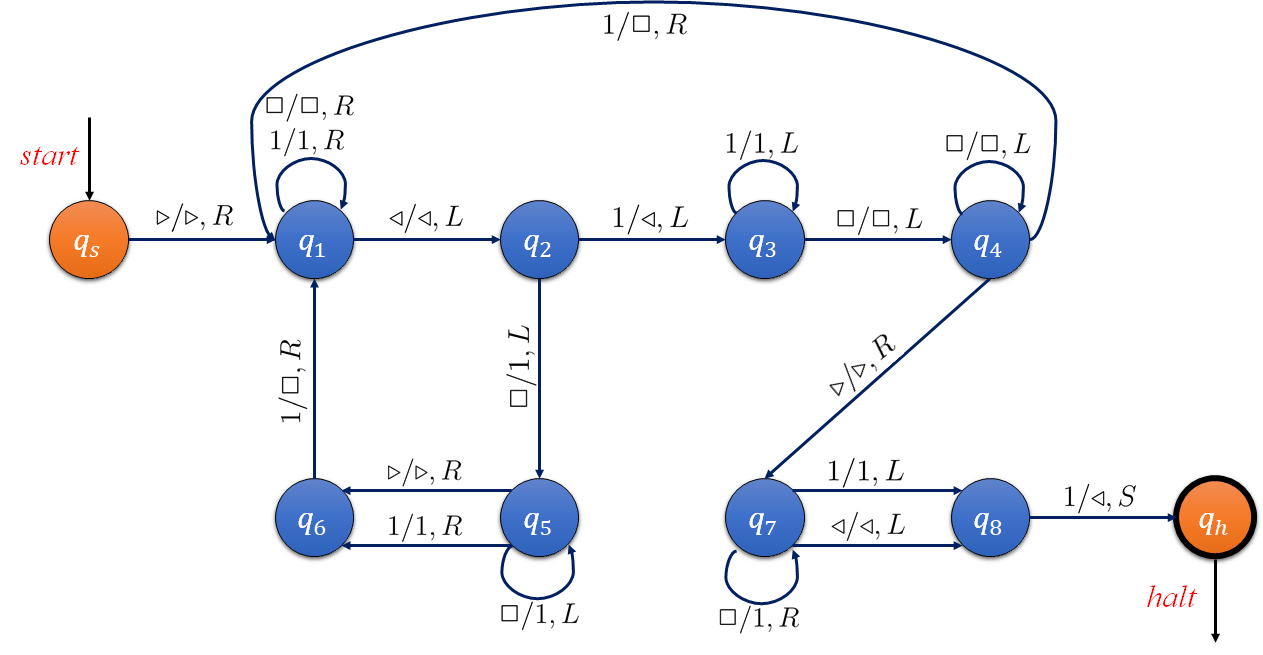
\includegraphics[width=6in]{state-transition-diagram.png}\\
  \caption{The state transition diagram}\label{fig1}
\end{figure}
\item The whole process from initial to final configurations for input $x = 7$ and $y = 3$ is as follows ({\color{blue}some useless parts of the tape are automatically ignored, and we will use the blue color to mark them one step before they are ignored}).
\begin{displaymath}
\begin{aligned}
 & \quad\ (q_s,\underline{\triangleright}  1  1  1  1  1  1  1  \Box 1  1  1   \triangleleft)
 \vdash (q_1,\triangleright  \underline{1}  1  1  1  1  1  1  \Box 1  1  1   \triangleleft)
 \vdash^* (q_1,\triangleright  1  1  1  1  1  1  1  \Box 1  1  1   \underline{\triangleleft}) \\
 & \vdash (q_2,\triangleright  1  1  1  1  1  1  1  \Box 1  1 \underline{1} \triangleleft)
 \vdash (q_3,\triangleright  1  1  1  1  1  1  1  \Box 1  \underline{1} \triangleleft {\color{blue}\triangleleft})
 \vdash^* (q_3,\triangleright  1  1  1  1  1  1  1  \underline{\Box} 1  1 \triangleleft) \\
 & \vdash (q_4,\triangleright  1  1  1  1  1  1  \underline{1} \Box 1  1 \triangleleft)
 \vdash (q_1, \triangleright  1  1  1  1  1  1  \Box \underline{\Box} 1  1 \triangleleft)
 \vdash^* \cdots \cdots \quad \textrm{\color{purple} (the same pattern (pattern 1)) } \\
 & \vdash^* (q_1,\triangleright  1  1  1  1  \Box  \underline{\Box} \Box \Box \triangleleft)
 \vdash^* (q_1,\triangleright  1  1  1  1  \Box  \Box \Box \Box \underline{\triangleleft})
 \vdash (q_2,\triangleright  1  1  1  1  \Box \Box \Box \underline{\Box} \triangleleft) \\
 & \vdash (q_5,\triangleright  1  1  1  1  \Box \Box \underline{\Box} 1 \triangleleft)
 \vdash^* (q_5,\triangleright  1  1  1  \underline{1} 1 1 1 1 \triangleleft)
 \vdash (q_6,\triangleright  1  1  1  1 \underline{1} 1 1 1 \triangleleft) \\
 & \vdash (q_1,\triangleright  1  1  1  1 \Box \underline{1} 1 1 \triangleleft)
 \vdash^* \cdots \cdots \quad \textrm{\color{purple} (the same pattern (pattern 2)) } \\
 & \vdash^* (q_1,\triangleright  1 \Box \underline{1} 1 1 \triangleleft)
 \vdash^* \cdots \cdots \quad \textrm{\color{purple} (the same pattern (pattern 1)) } \\
 & \vdash^* (q_1,\triangleright \Box  \underline{\Box} 1 1 \triangleleft)
 \vdash^* (q_1,\triangleright \Box  \Box 1 1 \underline{\triangleleft})
 \vdash (q_2,\triangleright \Box  \Box 1 \underline{1} \triangleleft)
 \vdash (q_3, \triangleright \Box \Box \underline{1} \triangleleft {\color{blue}\triangleleft})
 \vdash (q_3, \triangleright \Box \underline{\Box} 1 \triangleleft) \\
 & \vdash (q_4, \triangleright \underline{\Box} \Box 1 \triangleleft)
 \vdash (q_4, \underline{\triangleright} \Box \Box 1 \triangleleft)
 \vdash (q_7, \triangleright \underline{\Box} \Box 1 \triangleleft)
 \vdash^* (q_7, \triangleright 1 1 \underline{1} \triangleleft)
 \vdash (q_8, \triangleright 1 \underline{1} 1 \triangleleft) \\
 & \vdash (q_h, \triangleright 1 \underline{\triangleleft} {\color{blue}1 \triangleleft})
 \Rightarrow (q_h, \triangleright 1 \underline{\triangleleft})
\end{aligned}
\end{displaymath}
In the process above,
\begin{itemize}
\item pattern 1 means eliminating the last ``1'' of both $x$'s representation and $y$'s representation;
\item pattern 2 means eliminating $y$ ``1''s in $x$'s representation.
\end{itemize}

The final tape is $\cdots \triangleright 1 \underline{\triangleleft} \cdots$, which indicates $7\mod 3 = 1$, and it is correct.
\end{enumerate}
\end{solution}

\clearpage

\item Assume there's a Turing Machine $M$ using alphabet $\Gamma :\{ \triangleright, \Box, a, b, \cdots, z\}$. We can simulate $M$ by a Turing Machine $\tilde{M}$ using alphabet $\tilde{\Gamma }:\{ \triangleright, \Box, 0, 1\}$. Please transform the instruction $\langle q, i \rangle \rightarrow \langle q',j, R\rangle$ in $M$ into its corresponding form in $\tilde{M}$.
\begin{solution}
If we map $a,b,\cdots,z$ to $1,2,\cdots,26$ in order, then we need five $01$-bit to represent the letters. Thus, $i$ can be represented as $01001$, and $j$ can be represented as $01010$. Therefore, when using transition $\langle q, i \rangle \rightarrow \langle q',j, R\rangle$ in Turing Machine $\tilde{M}$, the initial tape state is as follows (Fig. \ref{fig2}).
\begin{figure}[htbp]
  \centering
  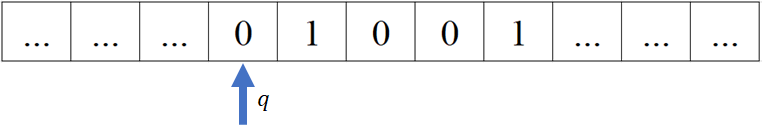
\includegraphics[width=2.3in]{initial-state.png}\\
  \caption{The initial tape state of $\tilde{M}$ before transition}\label{fig2}
\end{figure}

And the final tape state is as follows (Fig. \ref{fig3})
\begin{figure}[htbp]
  \centering
  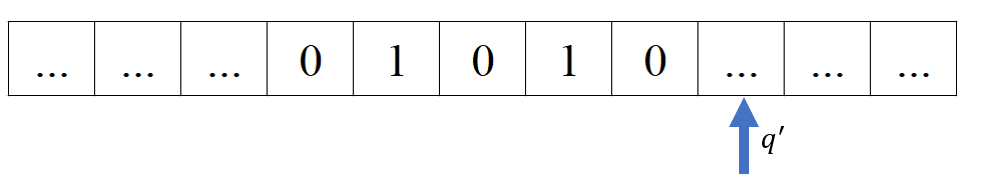
\includegraphics[width=2.3in]{final-state.png}\\
  \caption{The final tape state of $\tilde{M}$ after transition}\label{fig3}
\end{figure}

Here are the corresponding transitions of transition $\langle q, i \rangle \rightarrow \langle q',j, R\rangle$ in $\tilde{M}$.
\begin{displaymath}
\begin{aligned}
&\langle q, 0 \rangle \rightarrow \langle q^r_{0}, 0, R\rangle \qquad
&&\langle q^r_{0}, 1 \rangle \rightarrow \langle q^r_{01}, 1, R\rangle \qquad
&&\langle q^r_{01}, 0 \rangle \rightarrow \langle q^r_{010}, 0, R\rangle \\
&\langle q^r_{010}, 0 \rangle \rightarrow \langle q^r_{0100}, 0, R\rangle \qquad
&&\langle q^r_{0100}, 1 \rangle \rightarrow \langle q^r_{01001}, 1, S\rangle \qquad
&&\langle q^r_{01001}, 1 \rangle \rightarrow \langle q'^{wR}_{01010}, 1, S\rangle \\
&\langle q'^{wR}_{01010}, 0/1 \rangle \rightarrow \langle q'^{wR}_{0101}, 0, L\rangle \qquad
&&\langle q'^{wR}_{0101}, 0/1 \rangle \rightarrow \langle q'^{wR}_{010}, 1, L\rangle \qquad
&&\langle q'^{wR}_{010}, 0/1 \rangle \rightarrow \langle q'^{wR}_{01}, 0, L\rangle \\
&\langle q'^{wR}_{01}, 0/1 \rangle \rightarrow \langle q'^{wR}_{0}, 1, L\rangle \qquad
&&\langle q'^{wR}_{0}, 0/1 \rangle \rightarrow \langle q'^R_5, 0, S\rangle \qquad
&&\langle q'^R_5, 0/1 \rangle \rightarrow \langle q'^R_4, 0/1, R\rangle \\
&\langle q'^R_4, 0/1 \rangle \rightarrow \langle q'^R_3, 0/1, R\rangle \qquad
&&\langle q'^R_3, 0/1 \rangle \rightarrow \langle q'^R_2, 0/1, R\rangle \qquad
&&\langle q'^R_2, 0/1 \rangle \rightarrow \langle q'^R_1, 0/1, R\rangle \\
&\langle q'^R_1, 0/1 \rangle \rightarrow \langle q', 0/1, R\rangle
\end{aligned}
\end{displaymath}

We can divide the transitions above into three stages: \underline{reading stage, transition stage, writing stage} \underline{and moving stage}. Here are the reading stage, transition stage, writing stage and moving stage of the instruction $\langle q, i \rangle \rightarrow \langle q',j, R\rangle$ (Fig. \ref{fig4}, Fig. \ref{fig5}, Fig. \ref{fig6} and Fig. \ref{fig7}).
\begin{figure}[htbp]
  \centering
  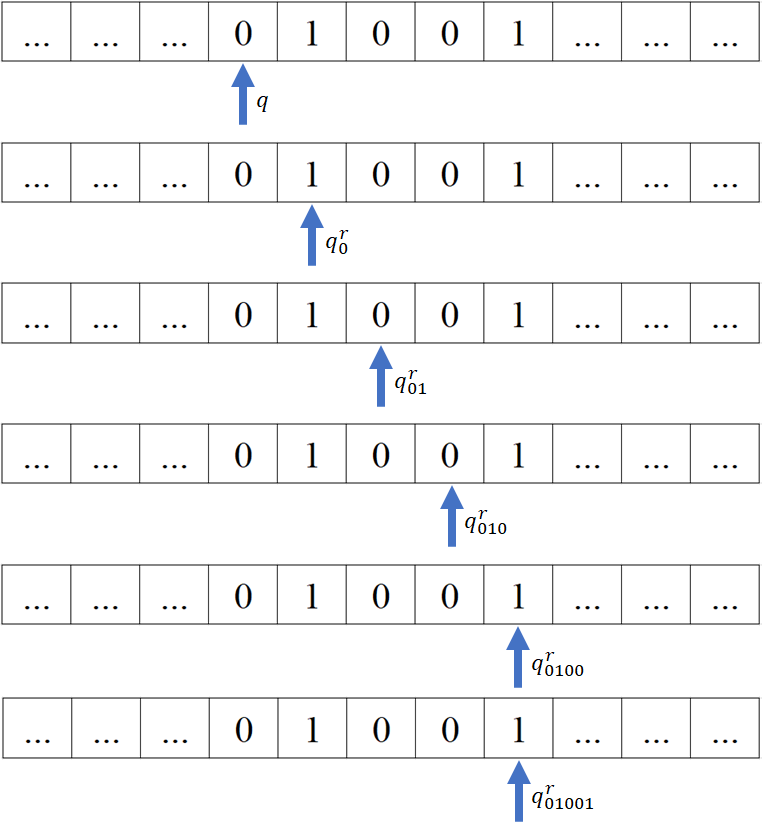
\includegraphics[width=2.3in]{reading-stage.png}\\
  \caption{The reading stage of the given instruction}\label{fig4}
\end{figure}
\clearpage
\begin{figure}[htbp]
  \centering
  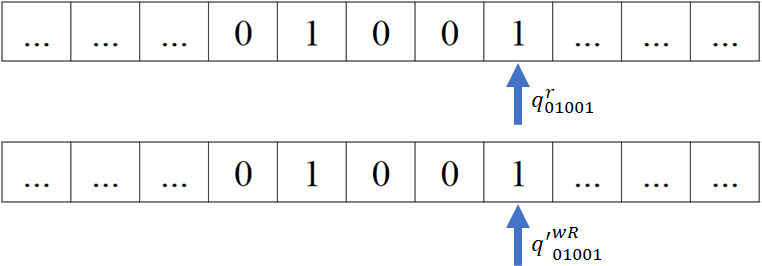
\includegraphics[width=2.3in]{transition-stage.png}\\
  \caption{The transition stage of the given instruction}\label{fig5}
\end{figure}
\begin{figure}[htbp]
  \centering
  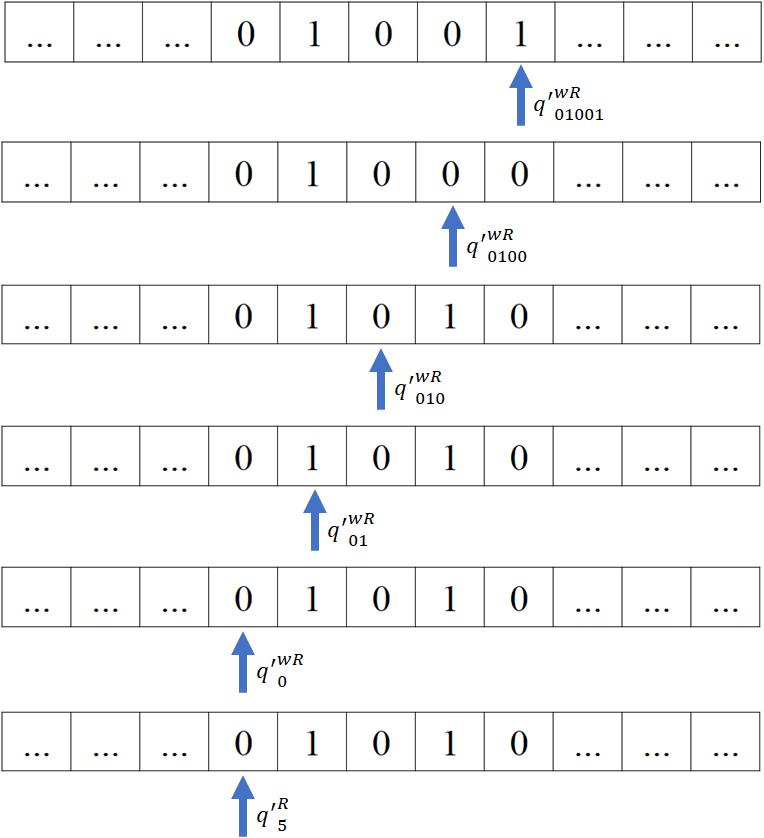
\includegraphics[width=2.3in]{writing-stage.png}\\
  \caption{The writing stage of the given instruction}\label{fig6}
\end{figure}
\begin{figure}[htbp]
  \centering
  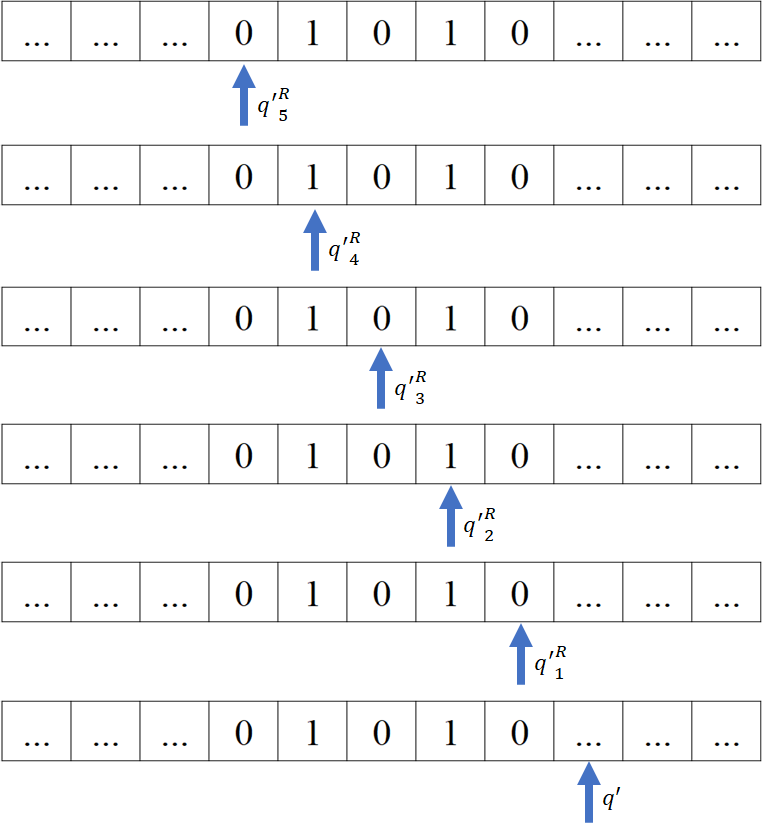
\includegraphics[width=2.3in]{moving-stage.png}\\
  \caption{The moving stage of the given instruction}\label{fig7}
\end{figure}

If we denote the five continuous blocks which contains the data as a \textit{macro-block}, then according the figures above, the reading stage is basically reading the data represented in macro-block; the transition stage is basically perform the corresponding transition of $M$ in $\tilde{M}$; the writing stage is basically writing the data to the macro-block; and the moving stage is basically moving to the next macro-block. Therefore, the transitions above of $\tilde{M}$ have the same function as the original transition $\langle q, i \rangle \rightarrow \langle q',j, R\rangle$ of $M$.
\end{solution}
\clearpage

\item \textbf{Wireless Data Broadcast System.}
In a Wireless Data Broadcast System (WDBS), data items are repeatedly broadcasted in cycle on different channels. Denote $D = \{d_1, d_2,\cdots, d_k\}$ as data items, each $d_i$ with length $l_i$ (as time units), and $\mathbf{C}=\{C_1, C_2, \cdots, C_n\}$ as broadcasting channels. Fig.~\ref{Fig-Broadcast} illustrates a WDBS with 25 data items and 4 channels. Once a channel finishes broadcasting current cycle, it will repeat these data again as a new cycle. E.g., a possible broadcasting sequence of $C_1$ could be \{$d_6$, $d_{12}$, $d_1$, $d_{18}$, $d_7$, $d_6$, $d_{12}$, $d_1$, $d_{18}$, $d_7$, $\cdots$\}

\begin{figure}[h]
	\centering
	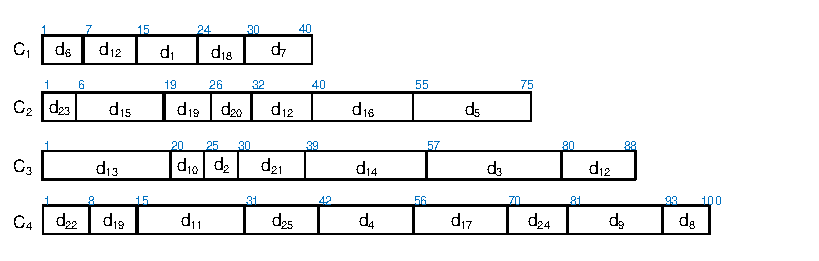
\includegraphics[scale=1]{Fig-Broadcast.pdf}
	\caption{An Example Scenario of Wireless Data Broadcast System.} \label{Fig-Broadcast}
\end{figure}

If a mobile client requires a subset of data items $D_q \subseteq D$ from this WDBS, he/she must access onto one channel, wait for the appearance of one required item, and switch to another channel if necessary. Each ``switch'' requires one time slot. For example, Lucien wants to download $\{d_1, d_3, d_5\}$, as shown in Fig.~\ref{Fig-Access}. He firstly accesses onto $C_1$ at time slot 1, then download $d_1$, $d_3$ respectively during time slots 2 to 5, and then switch to $C_3$ at time slot 6 (note that he cannot download $d_5$ from $C_2$ because of the switch constraint), and download $d_5$ during time slots 7 to 8. We define \emph{access latency} as the period when a client starts downloading, till the time he/she finishes. As a result, the overall access latency for Lucien is 7 in this example.

\begin{figure}[!htbp]
	\centering
	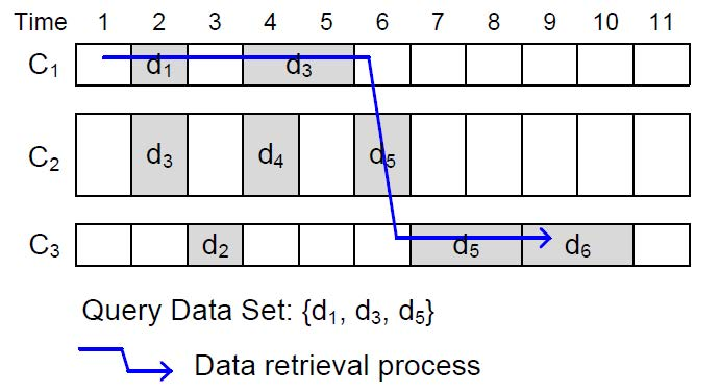
\includegraphics[scale= 0.5]{Fig-Access.pdf}
	\caption{An Example Scenario of Query of a Client.} \label{Fig-Access}
\end{figure}

Each operation (download/wait/switch) needs energy consumption. To conserve energy, a client hopes to use minimum amount of energy to download all required items in $D_q$, which means that he/she waits to minimize both access latency and switch numbers. Unfortunately, these two objectives conflict with each other naturally. Fig.~\ref{Fig-Conflict} exhibits such a scenario. To download $D_q=\{d_1, d_2, d_3, d_4\}$, if we start from $C_2$, in Option 1 we can switch to $C_1$ for $d_1$ immediately after downloading $d_3$, return back to $C_2$ for $d_4$, and to $C_1$ again for $d_2$. Such option costs 3 switches and 7 access latency. While in Option 2, we stay at $C_2$ lazily for $d_3$ and $d_4$, and then switch to $C_1$ for $d_2$ and $d_1$. Such option costs 1 switches and 12 access latency.
\clearpage

\begin{figure}[!htbp]
	\centering
	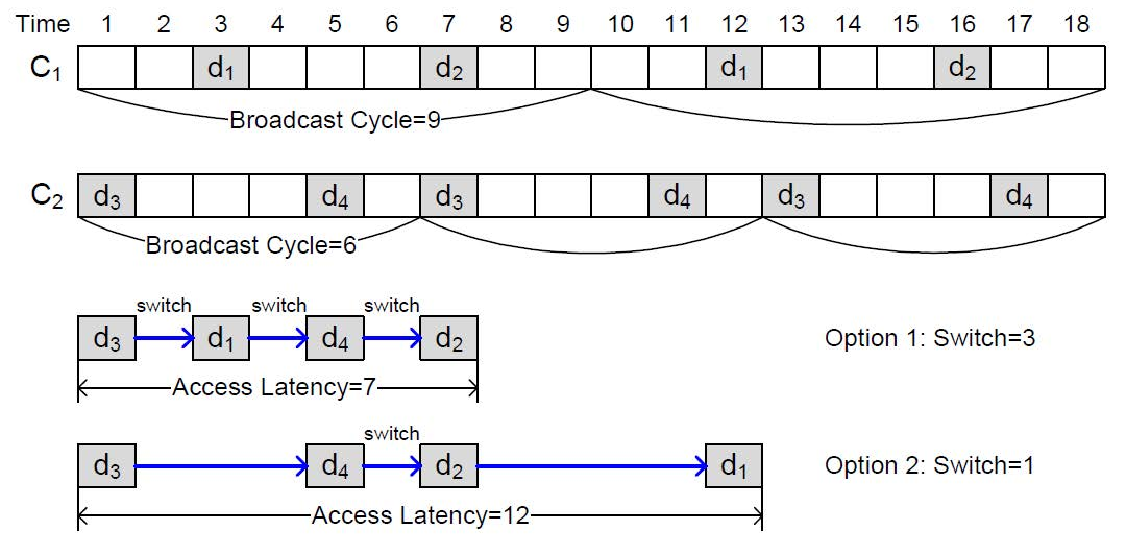
\includegraphics[scale= 0.5]{Fig-Conflict.pdf}
	\caption{Confliction between Access Latency and Switch Number.} \label{Fig-Conflict}
\end{figure}

Once we want to minimize two conflictive objectives simultaneously, we have three possible ways (similar as Segmented Least Squares told in Dynamic Programming Lecture). Now it is your turn to complete the formulation of this optimization, we name it as Minimum Constraint Data Retrieval Problem (MCDR), with the following sub-questions.
\begin{enumerate}
	\item If we add an additional switch parameter $h$, please define the MCDR (Version 1) completely as a search problem.
	\item If we add an additional latency parameter $t$, please define the MCDR (Version 2) completely as a search problem.
	\item If we set dimensional parameters $\alpha$ to switch number, and $\beta$ to access latency, we can combine two objectives together linearly as a new concept ``cost''. Please define the Minimum Cost Data Retrieval Problem (MCDR, Version 3) correspondingly.
	\item Please give the decision versions of sub-questions (a), (b) and (c).
\end{enumerate}

\begin{solution} Here are my answers to the sub-questions.
\begin{enumerate}
\item We make some definitions about switch and access latency first.
\begin{definition}[Switch]
A switch is changing the current channel to another channel, and it will cost one slot.
\end{definition}
\begin{definition}[Access latency]
Downloading each of the data items needs some time slots, and the number of time slots is equal to the length of the data item; every switch needs one time slot; we also need some extra time slots to waiting for target data items. The access latency is the sum of these time slots.
\end{definition}
Here is the definition of the search problem of MCDR (Version 1).
\begin{definition}[MCDR Version 1, Search Problem]
Given $k$ data items $D = \{d_1, d_2,\cdots, d_k\}$ located in $n$ different broadcasting channels $\mathbf{C}=\{C_1, C_2, \cdots, C_n\}$, and the target data items set $D_q \subseteq D$. Each data item $d_i$ has its length $l_i$, and it is located in some positions in some channels. Each channel has a different broadcast cycle length. Given a switch parameter $h$, then the \underline{Minimum Constraint Data Retrieval Problem} is to find a {\color{red}minimum access latency} data retrieval schedule under the constraint of at most $h$ switches.
\end{definition}
\item Here is the definition of the search problem of MCDR (Version 2).
\begin{definition}[MCDR Version 2, Search Problem]
Given $k$ data items $D = \{d_1, d_2,\cdots, d_k\}$ located in $n$ different broadcasting channels $\mathbf{C}=\{C_1, C_2, \cdots, C_n\}$, and the target data items set $D_q \subseteq D$. Each data item $d_i$ has its length $l_i$, and it is located in some positions in some channels. Each channel has a different broadcast cycle length. Given an access latency parameter $t$, then the \underline{Minimum Constraint Data Retrieval Problem} is to find a {\color{red}minimum switch number} data retrieval schedule under the constraint of at most $t$ access latency.
\end{definition}
\item Then we define the cost of a data retrieval schedule as follows.
\begin{definition}[Cost]
  Given a data retrieval schedule $S$, and two dimensional parameters $\alpha$ to switch number and $\beta$ to access latency. Suppose the switch number of the schedule $S$ is $h$, and the access latency of the schedule $S$ is $t$, then the cost $c$ of the schedule $S$ is defined as follows.
  \begin{displaymath}
  c \stackrel{\Delta}{=} \alpha h + \beta t
  \end{displaymath}
\end{definition}
Here is the definition of the search problem of MCDR (Version 3).
\begin{definition}[MCDR Version 3, Search Problem]
Given $k$ data items $D = \{d_1, d_2,\cdots, d_k\}$ located in $n$ different broadcasting channels $\mathbf{C}=\{C_1, C_2, \cdots, C_n\}$, and the target data items set $D_q \subseteq D$. Each data item $d_i$ has its length $l_i$, and it is located in some positions in some channels. Each channel has a different broadcast cycle length. Given two dimensional parameters $\alpha$ to switch number and $\beta$ to access latency, then the \underline{Minimum Cost Data} \underline{Retrieval Problem} is to find a {\color{red} minimum cost} data retrieval schedule.
\end{definition}
\item The decision versions of previous MCDR problems are as follows.
\begin{definition}[MCDR Version 1, Decision Problem]
Given $k$ data items $D = \{d_1, d_2,\cdots, d_k\}$ located in $n$ different broadcasting channels $\mathbf{C}=\{C_1, C_2, \cdots, C_n\}$, and the target data items set $D_q \subseteq D$. Each data item $d_i$ has its length $l_i$, and it is located in some positions in some channels. Each channel has a different broadcast cycle length. Given a switch parameter $h$ and an access latency parameter $t$, then the \underline{Minimum Constraint Data Retrieval} \underline{Problem} is whether there exists a data retrieval schedule whose {\color{red}access latency is no more than $t$}, under the constraint of at most $h$ switches.
\end{definition}
\begin{definition}[MCDR Version 2, Decision Problem]
Given $k$ data items $D = \{d_1, d_2,\cdots, d_k\}$ located in $n$ different broadcasting channels $\mathbf{C}=\{C_1, C_2, \cdots, C_n\}$, and the target data items set $D_q \subseteq D$. Each data item $d_i$ has its length $l_i$, and it is located in some positions in some channels. Each channel has a different broadcast cycle length. Given an access latency parameter $t$ and a switch parameter $h$, then the \underline{Minimum Constraint Data Retrieval} \underline{Problem} is whether there exists a data retrieval schedule whose {\color{red}switch number is no more than $h$}, under the constraint of at most $t$ access latency.
\end{definition}
\begin{definition}[MCDR Version 3, Decision Problem]
Given $k$ data items $D = \{d_1, d_2,\cdots, d_k\}$ located in $n$ different broadcasting channels $\mathbf{C}=\{C_1, C_2, \cdots, C_n\}$, and the target data items set $D_q \subseteq D$. Each data item $d_i$ has its length $l_i$, and it is located in some positions in some channels. Each channel has a different broadcast cycle length. Given two dimensional parameters $\alpha$ to switch number and $\beta$ to access latency and a cost parameter $c$, then the \underline{Minimum Cost Data Retrieval Problem} is whether there exists a data retrieval schedule whose {\color{red}cost is no more than $c$}.
\end{definition}
\end{enumerate}
\end{solution}
\end{enumerate}

%========================================================================
\end{document}
